\chapter{Introduction} \Contact{Alex}
\Contributors{Alex, Annika, Keith ...}
\label{sec:intro}
\bigskip

%\ADW{Do we need an executive summary? Should we rename ``Introduction'' to ``Executive Summary''?}\AHGP{I am down with relabeling this section as ``Executive Summary"} \ET{I agree the renaming idea is clearer} \ADW{We've added a separate executive summary that is more programmatically oriented.}

The fundamental nature of dark matter, which constitutes $\roughly 85\%$ of the matter density and 26\% of the energy density of the Universe, represents a critical gap in our understanding of fundamental physics.
Over the past several decades, experimental searches for particle dark matter have proceeded along several complementary avenues (\figref{interactions}).
Collider experiments (e.g., ATLAS and CMS at the Large Hadron Collider), attempt to produce and detect dark matter particles, while  %\citep{Boveia:2018yeb,Ehret:2010mh,Battaglieri:2017aum}
direct detection experiments (e.g., LZ, CDMS, ADMX, PICO, DAMiC, SENSEI, etc.) attempt to directly detect energy deposition from very rare scattering between dark matter and standard model particles.
%\citep{1509:02910, 1804.10697, Du:2018uak} 
%\AHGP{Cite only US experiments?} 
%\ADW{It was intentional, but perhaps ill advised...}
In parallel, indirect dark matter searches (e.g., {\it Fermi}-LAT, AMS-02, {\it Chandra}, XMM, etc.) seek to detect the energetic Standard Model products from the annihilation or decay of dark matter particles {\it in situ} in astrophysical objects. %\citep[\eg][]{1503.02641,1402.2301, 1605.01043, 1603.06978}. 
Despite these extensive efforts, the only robust, positive empirical measurement of dark matter continues to come from astrophysical and cosmological observations. 
% From the DOE DM BRN...
% The current global program of experiments using particle physics detectors, accelerators has yet to shine any light on the nature of dark matter.

%The search for dark matter particles is of high-priority to the particle physics community and a diversity of project scales should be maintained


%\AHGP{This paragraph is fairly WIMP-centric.  I added some axion- and hidden-photon-related refs.}

Astrophysics and cosmology offer a complementary technique to study the fundamental properties of dark matter. 
They probe dark matter directly through gravity, the only force to which dark matter is known to couple. On large scales, dark matter is well described by a simple model, the standard non-relativistic collisionless, stable cold dark matter (CDM) paradigm.
However, many viable theoretical models of dark matter predict observable deviations from CDM, which are testable with current and future experimental programs.
Fundamental properties of dark matter---e.g., particle mass, self-interaction cross section, coupling to the Standard Model, and time-evolution of dark matter properties---can imprint themselves on the macroscopic distribution of dark matter in a detectable manner.

%In addition, astrophysical observations complement particle physics searches by measuring the local distribution of dark matter, targeting indirect searches, and constraining the viable range of dark matter particle mass and electric charge.
%As the WIMP paradigm becomes more and more tightly constrained,  astrophysical observations will provide critical information to help direct the evolution of particle physics searches over the coming decade.  
%In many cases, observations with telescopes provide \emph{the only} robust, empirical constraints on the viable range of dark matter models.
%\AHGP{Alex, check my rewrite to see if I captured the essence of what you meant} \ADW{Thanks, tweaked a bit and looks good to me.}
In addition, astrophysical observations complement particle physics searches by providing input to direct and indirect dark matter searches, or by enabling alternative tests of dark matter's non-gravitational coupling to the standard mode.  
For example, astrophysical observations can be used to measure the local distribution of dark matter, an important variable for direct searches; can highlight regions of high dark matter densities for targeting indirect searches; and can identify astronomical objects that can lead to tight constraints the range of dark matter particle mass and electric charge for a specific dark matter model.  
Especially given that the dominant CDM particle model, the weakly interacting massive particle,  \citep[WIMP;][]{steigman1985}, becomes more and more tightly constrained, astrophysical observations will provide critical information to help direct the evolution of particle physics searches over the coming decade.  
In many cases, observations with telescopes provide \emph{the only} robust, empirical constraints on the viable range of dark matter models (\ie, the minimum mass of ultra-light dark matter).

At the same time, there is immense dark matter discovery potential at the intersection of particle physics and astrophysics.
Detecting a deviation from the gravitational predictions of CDM would provide much-needed experimental guidance on parameters that are not easily measured in particle physics experiments (\eg, dark matter self-interaction cross sections). 
If, on the other hand, all astrophysical studies of dark matter are found to agree with the CDM predictions, the improved knowledge of dark matter distributions will reduce major sources of theoretical uncertainties in the particle physics experiments. 
%ADW: I don't know what is being referred to here.
Likewise, results from particle experiments can either restrict the possible model space relevant to novel astrophysical signals, or suggest specific deviations from the CDM paradigm which can be tested with astrophysical observations.
The expanding landscape of new theoretical models for dark matter provides strong motivation to explore dark matter parameter space beyond the current sensitivity of the high-energy physics program.

The Large Synoptic Survey Telescope (LSST) is a next-generation wide-area optical survey instrument that will enable high-precision cosmological measurements to probe the fundamental physics of dark matter and dark energy \citep{0805.2366}. Following on predecessors such as the Sloan Digital Sky Survey (SDSS) and the Dark Energy Survey (DES), LSST promises to greatly enhance our knowledge of the dark sector of the Universe. 
LSST will measure the properties of dark matter over a wide range of astrophysical scales, and test a wide variety of particle physics models (\tabref{models}).
At the largest scales, LSST will use gravitational weak lensing and the large scale clustering of galaxies to trace the distribution of dark matter.
The profiles of dark matter halos associated with galaxies and clusters of galaxies can be used to test self-interacting dark matter models.
Measurements of the smallest scale clustering of dark matter in the faintest galaxies and gravitational perturbations in strong lensing and stellar tracers will enable constraints on warm and ultra-light dark matter.
In addition, the temporal component of the LSST ``wide, fast, deep'' survey will open a new window on the search for compact dark matter, such as primordial black holes (PBHs).
LSST will provide a rich scientific data set that can be used to develop novel and unanticipated constraints on dark matter properties through precise measurements of physical processes, such as anomalous energy loss in stars that could be produced by axions or axion-like particles.

In this white paper, we present several techniques that LSST will employ to probe the fundamental properties of dark matter. 
Rather than presenting a comprehensive review of astrophysical probes of dark matter  \citep[e.g.,][]{BuckleyPeter:2017} or an extensive discussion of any particular dark matter model \citep[e.g.,][]{Jain:2019}, we choose to focus on what we believe are some of the most exciting opportunities to study dark matter physics with LSST. 
Many astrophysical measurements require collaborative observations between several instruments, and the study of dark matter with LSST is no exception. 
Throughout this paper we describe situations where LSST will complement other astrophysical and particle investigations of dark matter.
Our over-arching goal in this paper is to convince our particle physics colleagues that not only will LSST provide exciting results on the nature of dark matter, but that observations from LSST are {\it essential} for guiding future particle physics searches.

\begin{figure}[t]
\centering
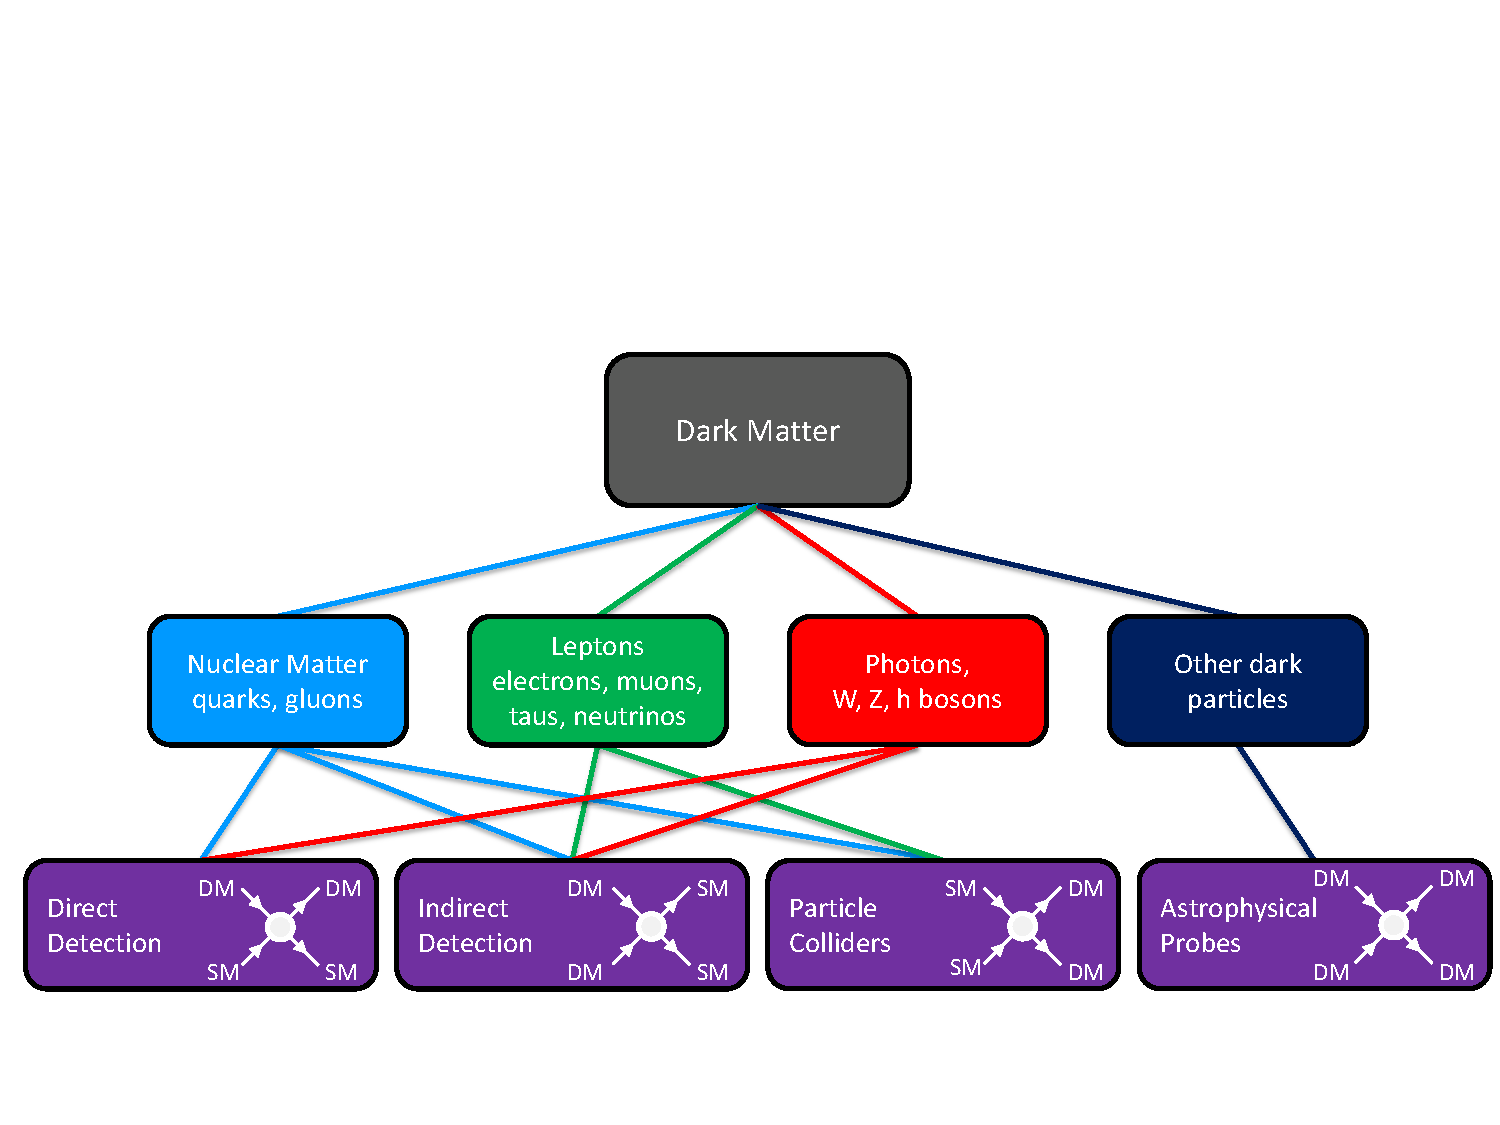
\includegraphics[width=0.85\textwidth]{figures/interactions.pdf}
\caption{
\label{fig:interactions}
Dark matter may have non-gravitational interactions that may be probed by four complementary approaches: 
direct detection, indirect detection, particle colliders, and astrophysical probes.
The lines connect the experimental approaches with the categories of particles that they most stringently probe (additional lines can be drawn in specific model scenarios). 
Figure taken from the Snowmass CF4 Report \citep{1305.1605}.
%\KB{Is it worth including a figure here to replace the ``conventional'' collider-direct-indirect dark matter search triangle? I'm thinking of something that people can easily re-use in talks and serves as a very simple visual to convey the importance of astrophysical probes.}\ADW{I've added this figure, but I'm not sure it's exactly what we want (we talk about non-gravitational interactions . It'd be good to hear Annika and Matt B.'s input, since I think they've thought about this a lot.}\AHGP{This is not a bad figure to use.  You can also use Matt \& my plot where we have a standard model interaction strength on on axis and a ``scale on which DM shouldn't look like CDM" scale on the other.  What that plot misses is the different types of standard-model and standard particle physics searches, but it puts particle and astro searches on the same footing.}
}
\end{figure}

\begin{table}[t]
\begin{center}
\begin{tabular}{l c c c}
\hline 
Model & Probe & Parameter & Value \\
\hline 
\hline
Warm Dark Matter (WDM) & Halo Mass & Particle Mass & \CHECK{$m_{\rm WDM} \sim 17 \keV$} \\
Self-Interacting Dark Matter (SIDM) & Halo Profile & Cross Section & \CHECK{$\sigma/m \sim 0.1\text{--}10\cm^2/\g$} \\
Baryon-Scattering Dark Matter (BSDM) & Halo Mass & Cross Section & \CHECK{$\sigma \sim 10^{-26} \cm^2$} \\
Axion-Like Particles (ALPs) & Energy Loss & Coupling Strength & \CHECK{$g_{\phi e} \sim 10^{-13} $} \\
Fuzzy Dark Matter (FDM) & Halo Mass & Particle Mass & \CHECK{$m \sim 10^{-21} \eV$}  \\
Primordial Black Holes (PBHs) & Compact Objects & Mass & \CHECK{$M \sim 10^{-12}\text{--}10^{7} \Msun$} \\
Weakly Interacting Massive Particles (WIMPs) & Indirect Detection & Cross Section & \CHECK{$\sigmav \sim 10^{-27} \cm^3/\second$} \\[+0.5em]
\hline
%\tablecomments{}
\end{tabular}
\end{center}
\caption{\label{tab:models} Probes of fundamental dark matter physics with LSST. \ADW{There are clearly a lot of caveats on each line, but I think that a table like this would be very useful. I could use help here!}\AHGP{I concur.}\FYCR{Yes, this is a good idea. Where does the 30 keV comes from?}}
\end{table}
